% !TEX TS-program = pdflatex
% !TEX encoding = UTF-8 Unicode
%\documentclass{article}

%\documentclass[ing,male,java,dept460,oneside]{diploma}
\documentclass{article}

\usepackage[czech]{babel}
\usepackage[T1]{fontenc} 
\usepackage[utf8]{inputenc}
\usepackage{color}
\usepackage{geometry}
\usepackage{float}
\usepackage{graphicx}
\usepackage{amsmath}
%\usepackage{amsthm}
\usepackage[stable]{footmisc}
\usepackage{hyperref}
\usepackage{amsfonts}
 \usepackage{bbm} 
 \usepackage{booktabs}
 \usepackage{url}
 
 
 
% \ThesisAuthor{Josef Raška}

% U bakalarske praxe neni nutne nazev zadavat
%\ThesisTitle{Tos ten android ze}

% U bakalarske prace neni nutne anglicky nazev zadavat
%\EnglishThesisTitle{The Android stuff}

%\SubmissionDate{29. dubna 2016}

%\PrintPublicationAgreement{true}


%\Thanks{Podekovani \newline Dalsi lajna }


%\CzechAbstract{Cesky abstrakt}

%\CzechKeywords{vlastní číslo, vlastní vektor, vlastní dvojice, aplikace vlastních čísel, mocninná metoda, Lanczosova metoda, předpodmínění}

%\EnglishAbstract{English abstract}

%\EnglishKeywords{Android, development}
 
\title{Bakalářská práce}
\author{Josef Raška \(ras0029\)}
\numberwithin{equation}{section}
\newtheorem{priklad}{Příklad}[section]
\newtheorem{veta}{Věta}[section]
\newtheorem{alg}{Algoritmus}[section]
\begin{document}
%\maketitle
%\MakeTitlePages
\urlstyle{same}

\tableofcontents
\listoffigures
\listoftables
%\lstlistoflistings

\newpage

\section{Úvod}

\section{Návrh aplikace}
\subsection{Popis aktérů}
\begin{figure}[H]
        \centering
                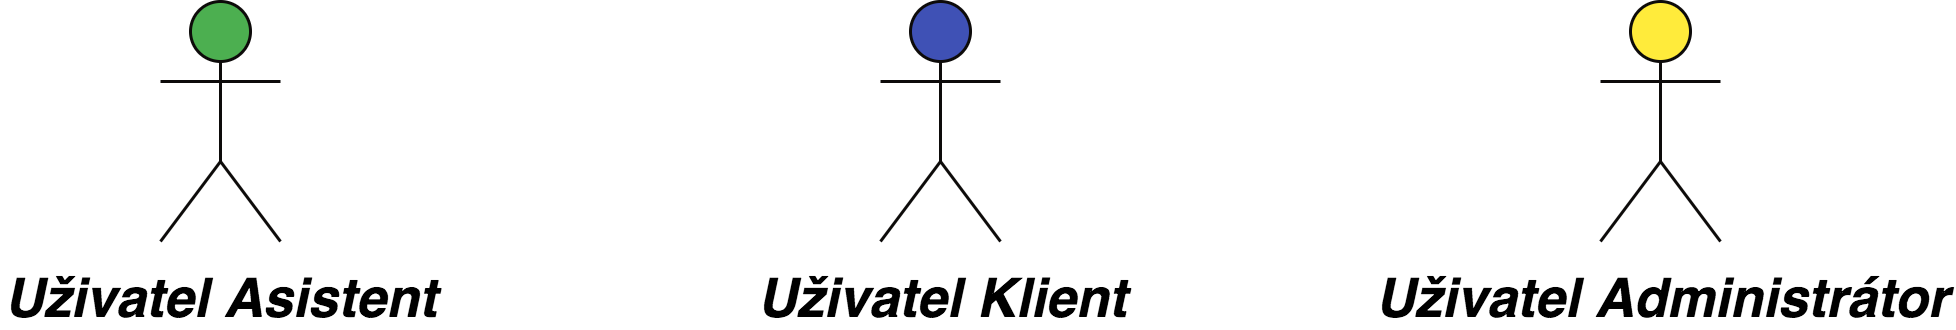
\includegraphics[scale=0.15]{img/actors.png}
        \caption{Aktéři systému}
        \label{fig:actors}
\end{figure}

\subsection{Use casy}
Pro uživatele klienta i asistenta jsou definovány případy užití zvlášť, neboť se celé chodvání
a použití aplikace bude v obou případech značně lišit.

\subsubsection{Uživatel asistent}
Pro uživatele asistnta jsou určeny složitější operace pro vytváření interaktivního obsahu pro klienta,
nastavování aplikace a prezentace klientovi. Pro use casy asistenta platí, že klient může těmto
krokům přihlížet, pokud o to projeví zájem.

\begin{figure}[H]
        \centering
                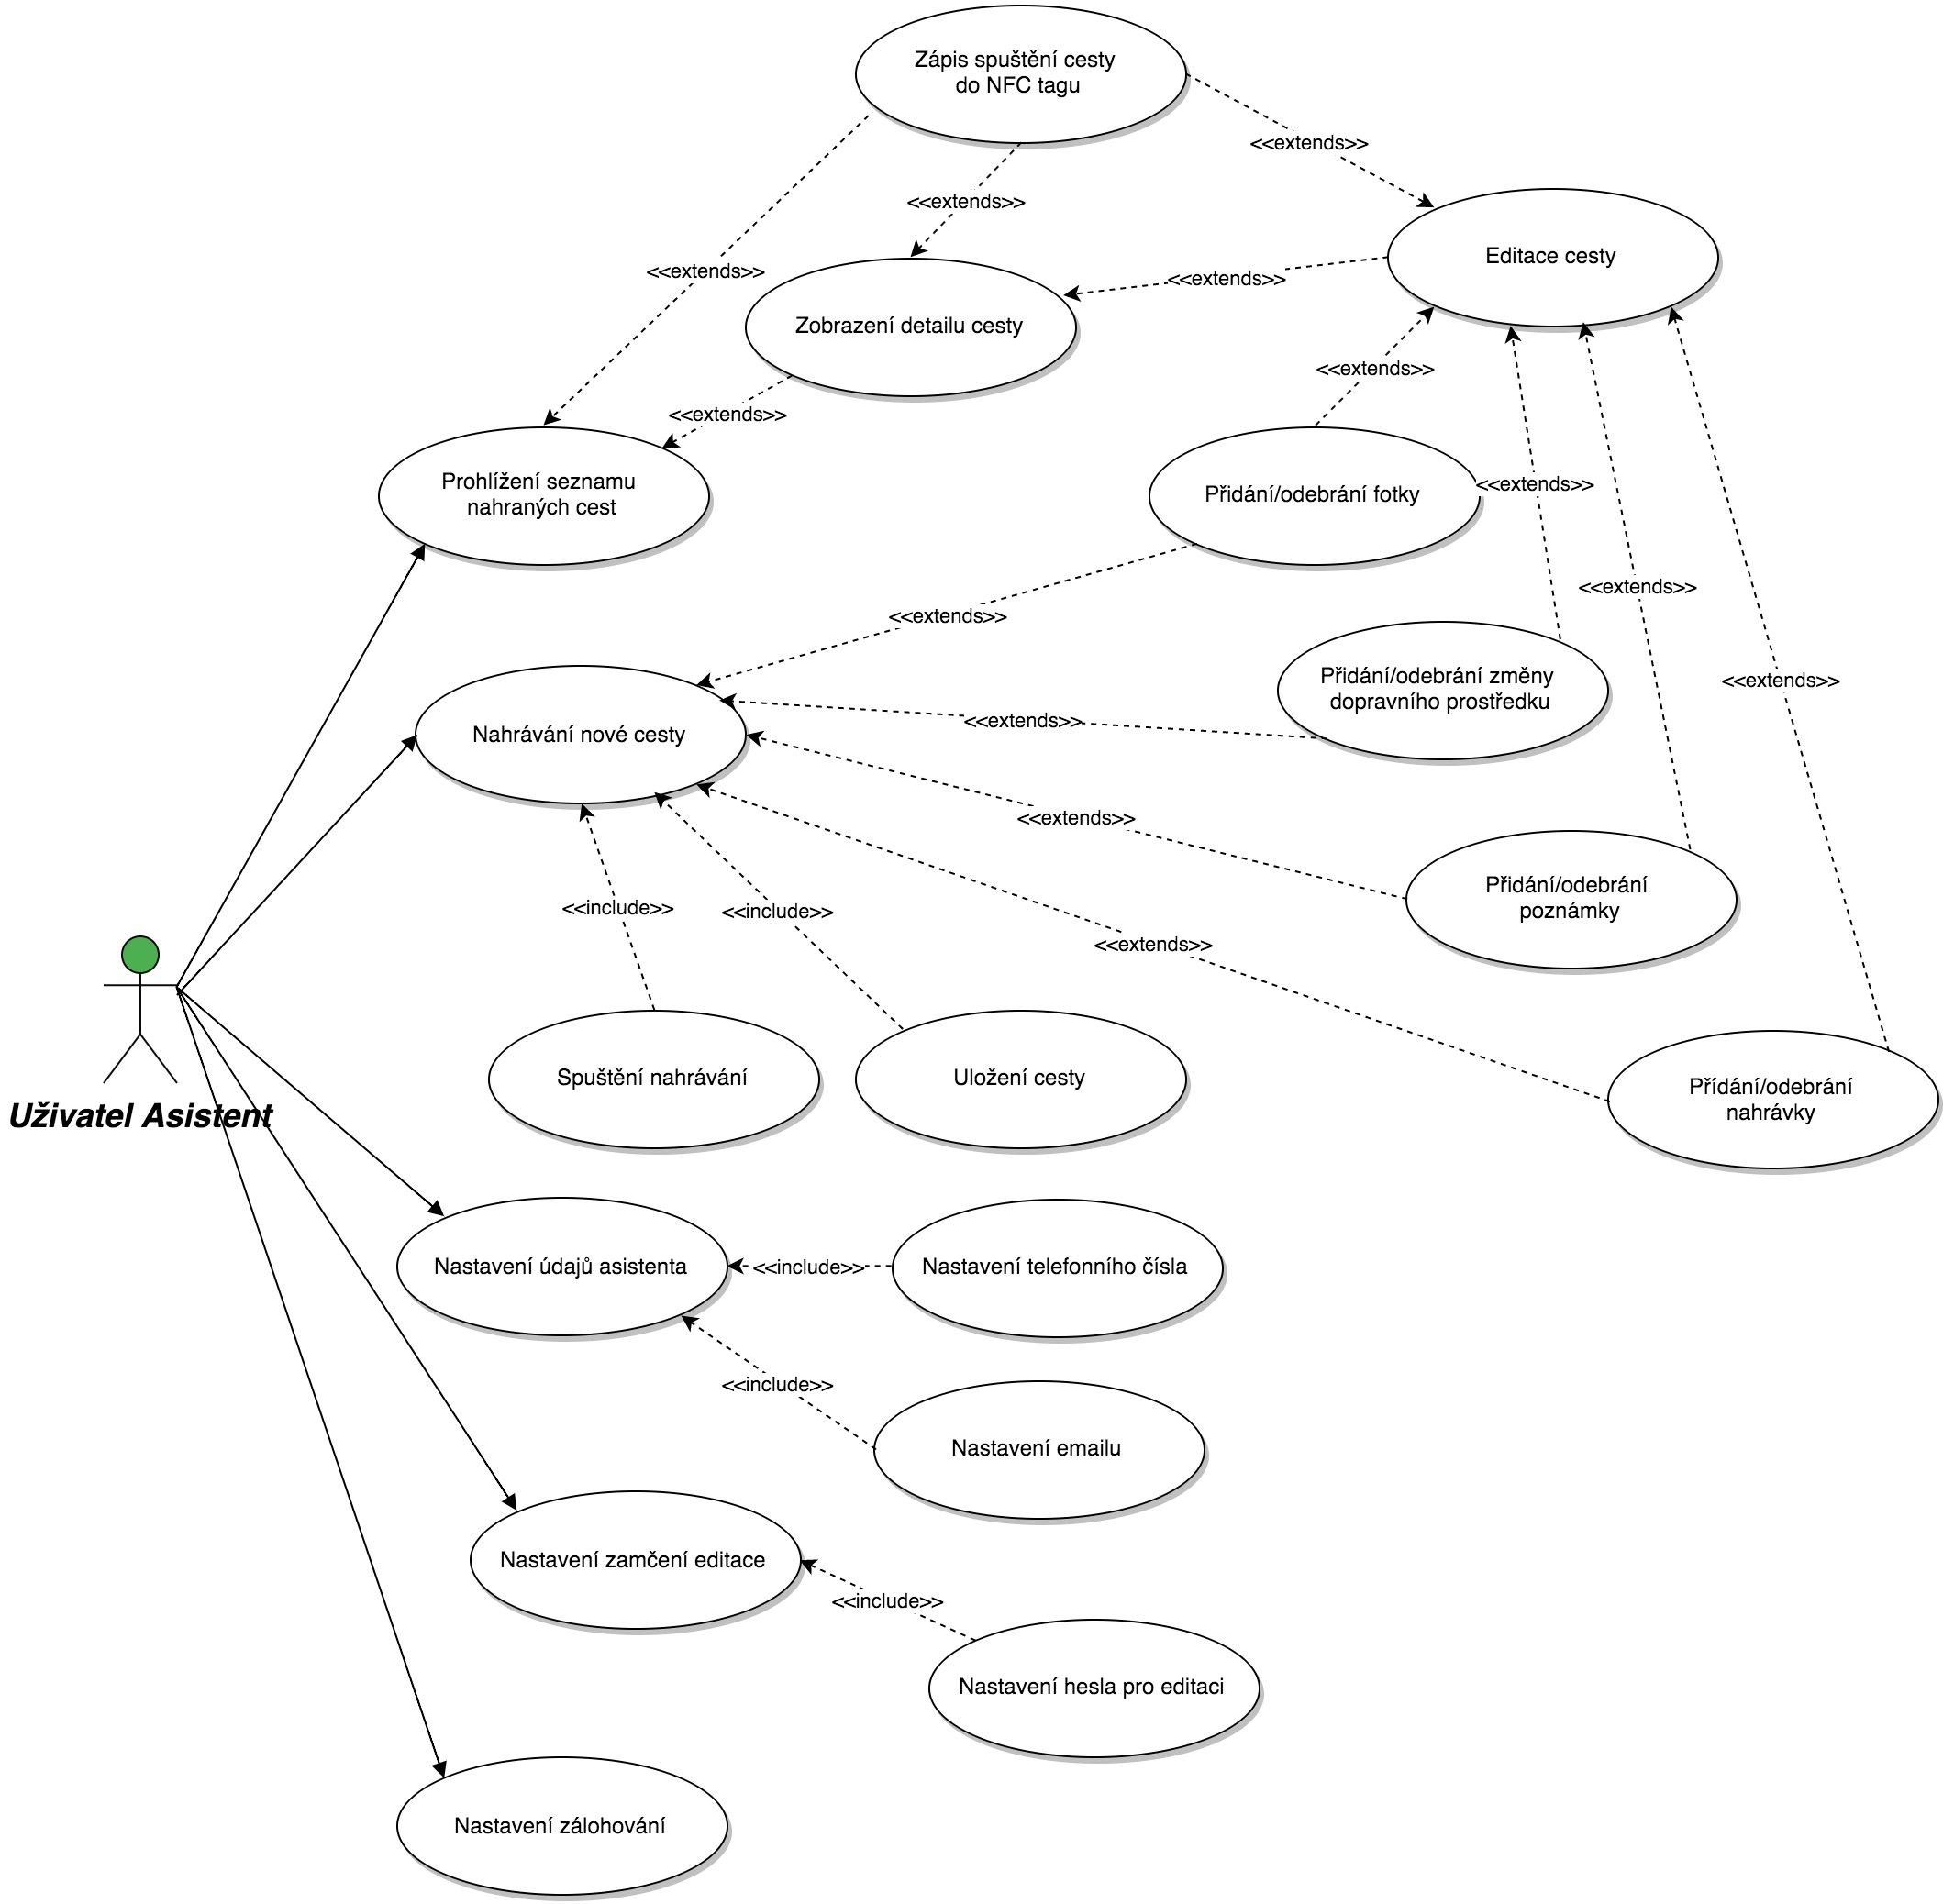
\includegraphics[scale=0.2]{img/UseCasesAsistant.png}
        \caption{Diagram use casů uživatele asistent}
        \label{fig:UseCasesAsistant}
\end{figure}

\subsubsection{Uživatel klient}
Pro klienta jsou určeny více intuitivní a nenáročné operace vyžadující co nejméně aktivních
kroků z klientovi strany. Aplikace by měla na základě polohy a dalších údajů sama rozpoznat,
co má v  danou chvíli udělat.

\begin{figure}[H]
        \centering
                \includegraphics[scale=0.2]{img/UseCasesClient.png}
        \caption{Diagram use casů uživatele klient}
        \label{fig:UseCasesClient}
\end{figure}

\subsection{Použité nástroje}
\subsubsection{draw.io (\url{http://www.draw.io})}
Online nástroj pro tvorbu grafů, všech různých typů diagramů, myšlenkových map a dalších.
Celý edior běží pouze v prohlížeči a synchronizuje vytvářené grafy s připojeným úložištěm
Google Drive nebo Dropbox. Grafy jsou tak přístupné  a editovatelné odkudkoliv a aplikace
je opravdu pokročilá a při práci není vůbec poznat, že vše probíhá pouze v prohížeči.
Umožňuje sdílení i export zhotovených diagramů do mnoha formátů a je tedy velice snadné
sdílet a používat vytvořenou práci.
Nástroj byl použit pro vytváření use case diagramů a třídnách diagramů v této práci.
\begin{figure}[H]
        \centering
                
\includegraphics[scale=0.2]{img/drawiologo.png}
        \caption{Logo nástroje draw.io}
        \label{fig:iologo}
        \centering Zdroj: \url{http://www.draw.io}
\end{figure}

%\subsection{Podnadpis\footnote{Inspirace v \cite{saad}}}



\section{Závěr}


\begin{thebibliography}{99}

\end{thebibliography}

  \appendix

  \section{Zdrojové kódy}
  Kódy lze nalézt i na přiloženém CD.

\end{document}